% -*- coding: utf-8 -*-

\section{决策树}
% https://en.wikipedia.org/wiki/Decision_tree
\subsection{直观印象}
\begin{frame}
    \begin{figure}[!tb]
        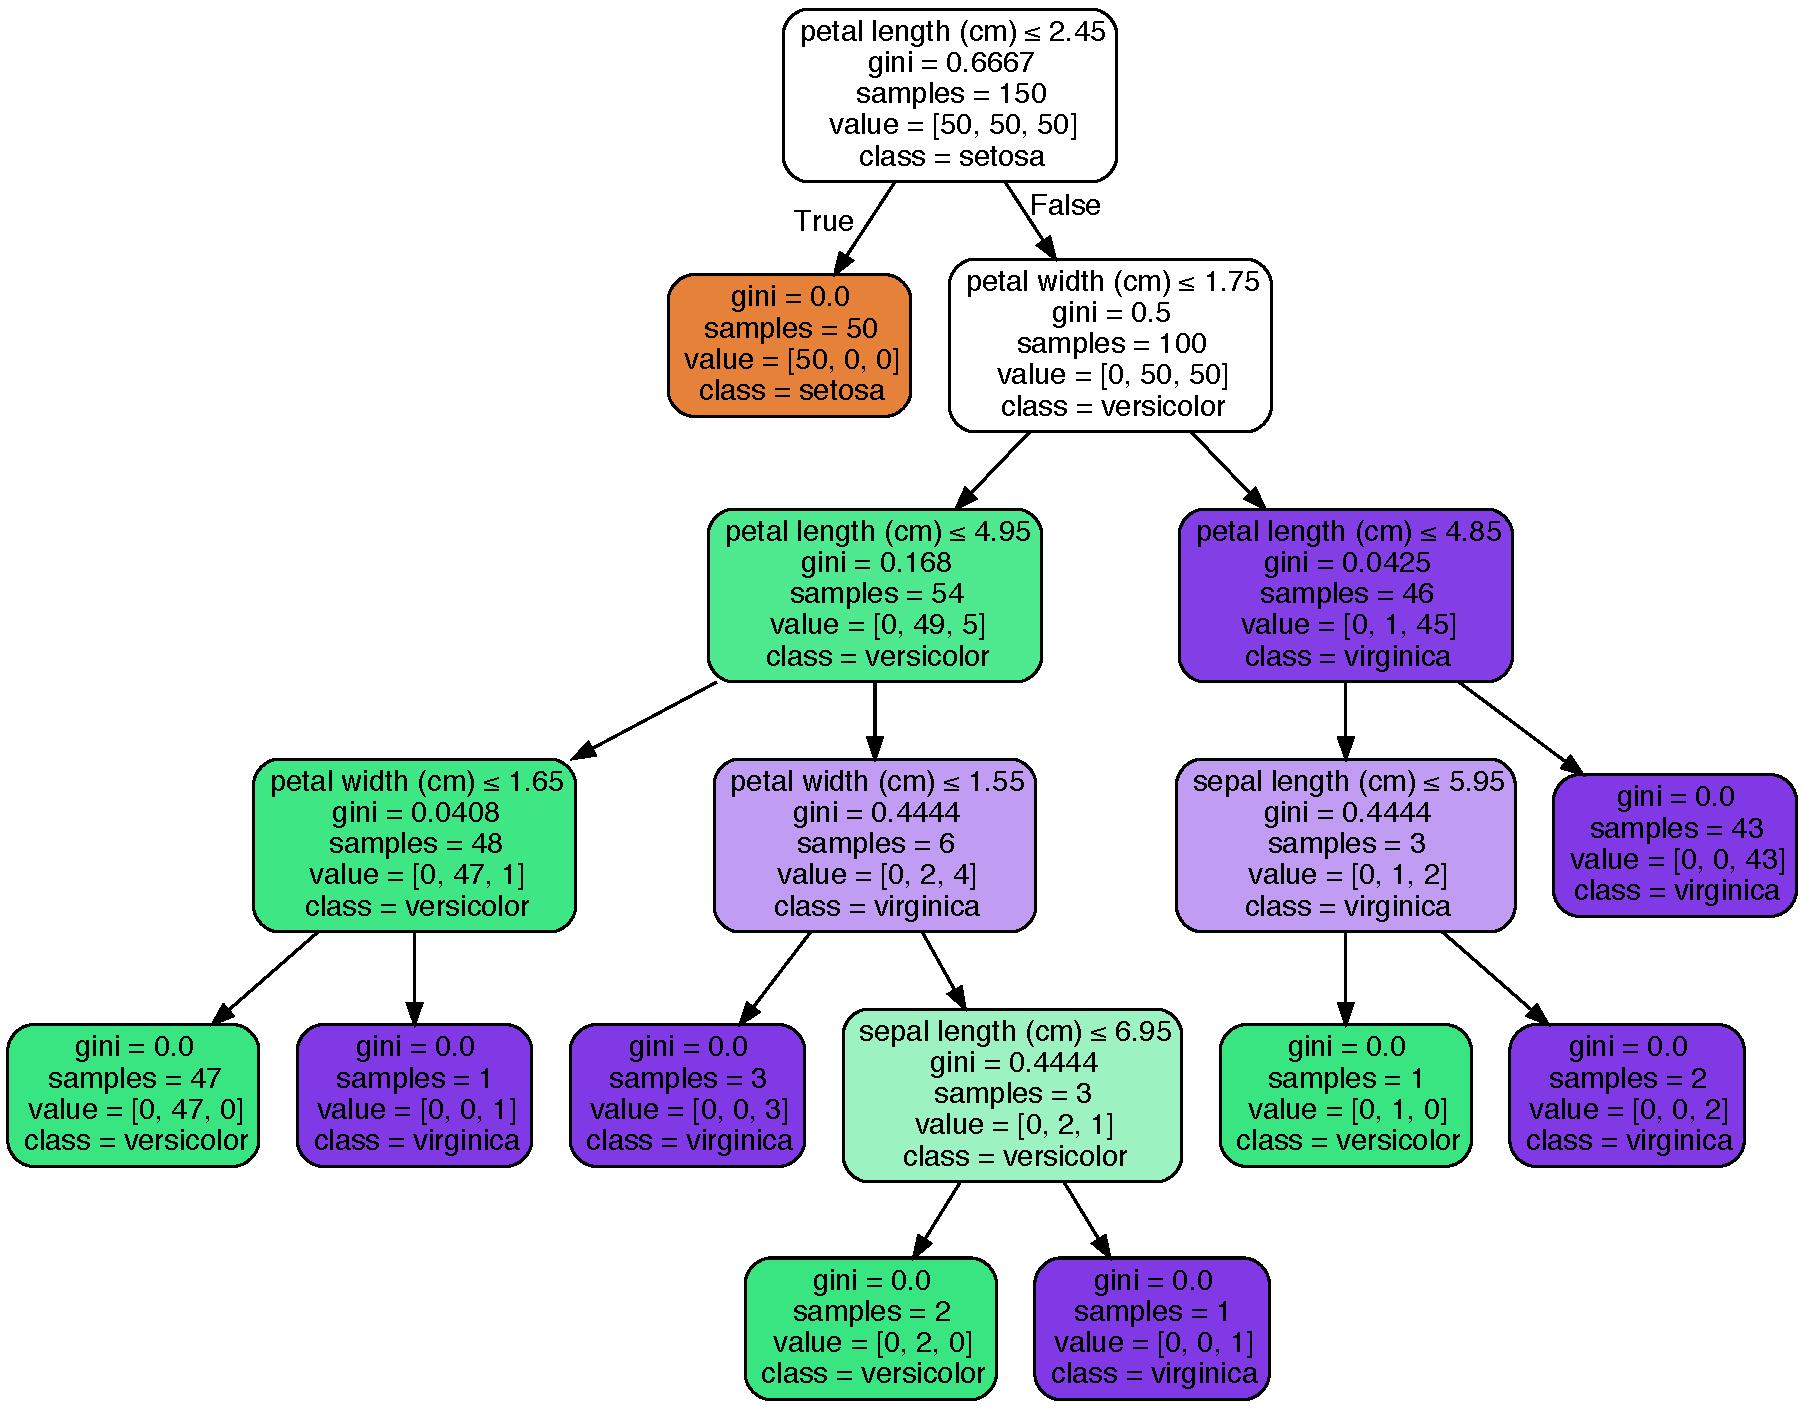
\includegraphics[width=\onepicwidth]{figure/decision_tree/iris}
        \caption{决策树示意\footnote{
                 \href{http://scikit-learn.org/stable/modules/tree.html}{Decision trees of iris data, scikit-learn}}}
    \end{figure}
\end{frame}

%\subsection{变种实现}
% ID3, C4.5
% split critor
%% 三种纯净度,图

%\subsection{CART}
% regression tree
%% binary -> possibility,实现
%% 用pandas,sklearn训练一个,看看输出概率值,集中在0和1两个极值处

\subsection{进化分支}
% http://www.cnblogs.com/LeftNotEasy/archive/2011/03/07/random-forest-and-gbdt.html
\begin{frame}{集成方法(Ensemble Method)}
    \begin{figure}[!tb]
        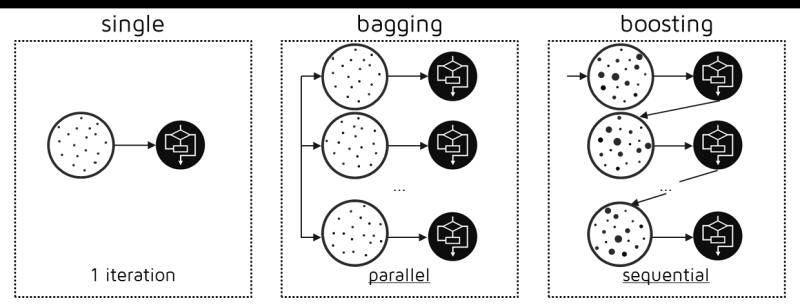
\includegraphics[width=.8\linewidth]{figure/decision_tree/bag_boost}
        \caption{Bagging和Boosting示意\footnote{
                 \href{http://quantdare.com/2016/04/what-is-the-difference-between-bagging-and-boosting/}{What is the difference between Bagging and Boosting, xristica}}}
    \end{figure}
\end{frame}

% 文献引用
